\documentclass{article}
\usepackage{lmodern}
\usepackage[utf8]{inputenc}
\usepackage[T1]{fontenc}
\usepackage[czech]{babel}
\usepackage{hyperref}
\usepackage[pdftex]{graphicx}

\ifpdf
\hypersetup{
	pdfauthor={Ondřej Profant},
	pdfsubject={Podrobná specifikace zápočtového programu z~Neproceduralniho programovani (NPRG005) na MFF UK},
	pdftitle={Specifikace zápočtového programu z~Neprocedurálního programování},
	pdfkeywords={NPRG005,PROLOG,SWI,CHEMIE,Anorganicka chemie,MFF},
}
\fi
\title{Specifikace zápočtového programu z~Neprocedurálního
programování (NPRG005)}

\author{Ondrej Profant}
\date{2011-05-06}

\begin{document}

\begin{center}
\LARGE
Specifikace zápočtového programu z~Neprocedurálního
programování (NPRG005)

\vspace*{2cm}

\large
programuje Ondřej Profant pod vedením Rudolfa Kryla\\
na MFF UK

\vspace{2cm}

\today

\vspace{2cm}
\end{center}

\normalsize
Cílem je udělat program pro práci s~převážně anorganickou chemii. Čili
implementovat:

\begin{enumerate}
\item periodickou tabulku prvků se základními informacemi o~prvcích 
\item převod z~vzorce na české chemické názvosloví (co$_2$ ={\textgreater}
oxid uhličitý)
\item převod z~českého názvosloví na vzorce (opačný k~bodu 2)
\item doplňování možných alternativ ve vzorcích a názvech 
\item základy organické chemie
\end{enumerate}
Nazval jsem jej AllCHEMIE.

\clearpage

\tableofcontents

\clearpage
\section{Implementační detaily}
Implementace bude v~jazyku Prolog v~dialektu SWI (viz. [4]). Nebudou využívány žádné
knihovny 3. stran.

\subsection{Struktura kódu}
Celý program bude rozdělen do souborů dle logických souvislostí, např.
v~souboru \texttt{periodic.table.pl} bude databáze prvků, predikáty pro
dotazování nad prvky, databáze koncovek a dalších zcela základních věcí
pro obor chemie.

V~dalších souborech budou predikáty pro různé sloučeniny a pravidla
jejich převodu, které díky vhodnosti Prologu pro tyto úlohy budou
srozumitelné i pro poučeného (snažícího se) laika.

Všechny predikáty budou koncipovány tak, aby šlo kterýkoliv argument
vynechat (zapsat jako proměnnou) a tím získat seznam možných
sloučenin / názvů / prvků. Tato vlastnost samozřejmě bude využívat základní
stavební prvek Prologu a bude tento program odlišovat od obdobných
např. webových aplikací. 

\subsection{Ovládání}
Nebude implementovaná diakritika a česká morfologie a program bude
výsledky uvádět pouze ve tvaru:

\texttt{oxid uhlik-icity}

\texttt{kyselina dihydrogen sira-ova}

\medskip

Pro všechny sloučeniny bude jeden základní predikát, který si sám
rozliší o~co se jedná, např:

\texttt{vstup(c,o,2).  /* dotaz na oxid uhlicity */}

\texttt{vstup(h,2,s,o,4).  /* dotaz na kyselinu sirovou */}

\subsection[Anorganická chemie]{Anorganická chemie}
Z~anorganické chemie bude implementována SŠ látka: oxidy, peroxidy,
kyslíkaté kyseliny, bezkyslíkaté kyseliny, halogenidy, sloučeniny
vodíku, soli. 

\subsection[Organická chemie]{Organická chemie}
Organická chemie je rozsáhlá a vyžaduje mnoho druhů vzorců.\footnote{[2] udává 6 typů vzorců, některé látky jsou bez správného typu vzorce nerozlišitelné.} Proto z~ní implementuji pouze základní lineární řadu s~jednoduchými vazbami: metan, propan, butan, \ldots a jejich uhlíkové zbytky (metyl, propyl, ethyl).

\section{Uživatelské rozhraní}
Uživatelské rozhraní bude interaktivní textové, ovládat se bude dle
několika základních predikátů.


\begin{center}
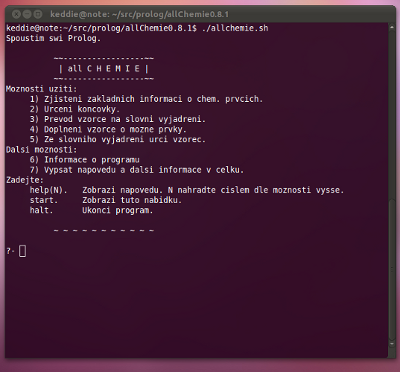
\includegraphics[scale=1]{allchemie-screen.png}
Obrázek 1: Předběžná ukázka rozhraní programu
\end{center}

\section{Dokumentace}
Velký důraz bude kladen na uživatelskou dokumentaci, jelikož program
bude pracovat přímo v~interaktivním modu Prologu a uživatel ho bude
moci ovládat pouze skrz několik málo predikátů. 

Přítomná bude rozsáhlá interaktivní nápověda přímo v~programu.

Uživatelská příručka bude obsahovat velké množství příkladů, které
pomohou k~pochopení používání a možností, které program bude nabízet.
Samozřejmostí je popis instalace a spuštění na několika platformách.

Programátorská dokumentace naopak již bude relativně prostá, neb
implementace by měla být přímočará (s~žádnými „špeky“ a záhadnými
predikáty o~kterých nikdo neví, co dělají).

\section{Literatura a další zdroje}
Vzhledem k~převážné odbornosti programu se přímo v~kódu odkazuji na
použité zdroje, např:

\texttt{member(M,[1,2,3,4,5,6,7,8]),  /* dle PSCH [1] str. 160 */}

\subsection{Knižní}
\begin{description}
\item[[1]] Přehled středoškolské chemie, vydalo SPN, Praha 1999 (kolektiv)
\item[[2]] Přehled středoškolského učiva chemie, ing. Ludvík Kosina, ing.
Vratislav Šrámek, vydala Albra 1995
\end{description}
\subsection{Software}
\begin{description}
\item[[3]] Gperiodic, GTK periodická tabulka prvků, homepage:\\
\hyperlink{http://www.frantz.fi/software/gperiodic.php}{http://www.frantz.fi/software/gperiodic.php} (odkaz k~6. 5. 2011)
\item[[4]] SWI-Prolog, použitá implementace Prologu, homepage:\\
\hyperlink{http://www.swi-prolog.org/}{http://www.swi-prolog.org/} (odkaz k~6. 5. 2011)
\end{description}
\subsection[Internetové]{Internetové}
\begin{description}
\item[[5]] Chem-web: \hyperlink{http://www.chem-web.info}{http://www.chem-web.info} (odkaz k~6. 5. 2011)
\end{description}

\end{document}
